\chapter{Background Information}

This chapter describes key concepts of data provenance, IoT characteristics, and provenance models. It outlines the tradeoffs that exists between provenance, log data and metadata. 

\section{Data Provenance}
The Oxford English dictionary defines provenance \cite{TCDP1999} as ``the place of origin or earliest known history of something."  An example of provenance can be seen with a college transcript. A transcript is the provenance of a college degree because it outlines all of the courses satisfied in order to attain the degree.
\par In the field of computing, data provenance, also known as  data lineage, can be defined as the history of all activities performed on entities from its creation to its current state. Cheney et al. \cite{cheney_provenance_2009} decribes provenance as the origin and history of data from its lifecycle. Buneman et al \cite{buneman_why_2001} describes provenance from a database perspective as the origin of data and the steps in which it is derived in the database system.  We formally define provenance as follows:


\begin{definition}

Data provenance of an entity is a comprehensive history of activities that occur on that entity from its creation to its present state.

\end{definition}

Provenance involves two granularity levels: fine-grained provenance and coarse-grained provenance. Fine-grained provenance \cite{glavic_case_2011} entails the collection of a detailed level of provenance. Coarse grained provenance, on the other hand, is a collection of a summarized version of provenance. Data provenance has immense applications and has been explored in the areas of scientific computing \cite{groth, altintas} to track how an experiments are produced, in business to determine the work-flow of  a process, and in computer security for forensic analysis and intrusion detection \cite{bates_towards_2013, muniswamy_reddy_provenance_2010, muniswamy_reddy} . Provenance denotes the who, where and why of data \cite{cheney_provenance_2009}. An example of provenance for a software system is a web server's log file. This file contains metadata for various request and response time and the ip address of all host systems that requests information from the server. This log file identifies the data object(i.e Web server), transformations that occurs on this object (e.g read write connections) and the state of the data object. Provenance data is represented as an acyclic graph which denotes casual relationship and dependencies between entities. Figure 1 illustrates an example from our use case of provenance above. It outlines a graphical representation of relationships contained in a server's log file.


%instert picture!!!


\par Provenance ensures trust and integrity of data \cite{Bertino2015}. It outlines causality and dependency between all objects involved in the system and allows for the verification of the source of data. Causality and dependency are used to determine the relationship between multiple objects. The relationship in which provenance denotes can in turn be used in digital forensics \cite{zawoadfecloud} to investigate the cause of a malicious attack and also in intrusion detection systems to further enhance the security of computing devices. 
 



%\subsection{Provenance-system collection}
%
%\subsubsection{Observed Provenance}
%
%\subsubsection{Disclosed Provenance}



\subsection{Provenance Characteristics}

Since provenance denotes the who, where and why of data transformation, it is imperative that data disseminated in an IoT architecture satisfies the required conditions. The characteristics of data provenance are outlined in detail below.


\begin{itemize}

\item Who: This characteristic provides information on activities made to an entity. Knowing the ``who" characteristic is essential because it maps the identity of modification to a particular data object. An example of ``who" in an IoT use case is a sensor device identifier.

\item Where: This characteristic denotes location information in which data transformation was made. This provenance characteristic could be optional since not every data modification contains location details.

\item When: This characteristic denotes the time information at which data transformation occurred. This is an essential provenance characteristic. Being able to tell the time of a data transformation allows for tracing data irregularities.

\item What: This characteristic denotes the transformation is applied on a data object. A use case for IoT can be seen in the various operations (create, read, update, and delete) that could be performed on a file object.

\end{itemize}


 
\section{Internet of Things (IoT)}
There is no standard definition for IoT, however, researchers have tried to define the concept of connected ``things". The concept of IoT was proposed by Mark Weiser in the early 1990s \cite{Mattern} which represents a way in which the physical objects, ``things", can be connected to the digital world. Gubbi et al \cite{park_provenance-based_2012} defines the IoT as  an interconnection of sensing and actuating devices that allows data sharing across platforms through a centralized framework. We define (IoT) as follows:

\begin{definition}
The Internet of Things (IoT) is a network of heterogeneous devices with sensing and actuating capabilities communicating with each other. 

\end{definition}

The notion of IoT has been attributed to smart devices. The interconnectivity between various heterogeneous devices allows for devices to share information in a unique manner. Analytics is a driving force for IoT. With analytics, devices can learn from user data to make smarter decisions. This notion of smart devices is seen in various commercial applications such as smartwatches, thermostats that automatically learns a user patterns. The ubiquitous nature of these devices make them ideal choices to be included in consumer products. IoT architecture consists of four distinct layers: The sensor and actuator layer, device layer, gateway layer and the cloud layer. 

\par With the recent data explosion \cite{emc_bigdata} due to the large influx in amounts of interconnected devices, information is disseminated at a fast rate and with this increase involves security and privacy concerns. Creating a provenance-aware system is beneficial to IoT because it ensures the trust and  integrity of interconnected devices. Enabling provenance collection in IoT devices allows these devices to capture valuable information which enables backtracking in an event of a malicious attack. We take a holistic approach to provenance collection by looking at how provenance information is collected across an IoT architectural framework.

 
  \subsection{IoT Architecture}

IoT architecture represents a functional hierarchy of how information is disseminated across multiple hierarchies contained in an IoT framework; from devices which contain sensing and actuating capabilities to massive data centers (cloud storage). Knowing how information is transmitted layers allows a better understanding on how to model the flow of information across actors contained in an IoT hierarchy. 
\par Figure \ref{iot_architecture} displays the IoT architecture and the interactions between the respective  layers. The base of the architectural stack consist of sensors and actuators which gathers provenance information and interacts with the device layer. The device layer consists of devices (e.g mobile phones, laptops, smart devices) which are responsible for aggregating data collected from sensors and actuators. These devices in turn forwards the aggregated data to the gateway layer. The gateway layer routes and forwards data collected from the device later. It could also serve as a medium of temporary storage and data processing. The cloud layer is involved with the storage and processing of data collected from the gateway layer. Note that the resource constraints decreases up the architectural stack with the cloud layer having the most resources (memory, power computation) and the sensor-actuator layer having the least. 


\begin{figure}[h]
\begin{center}

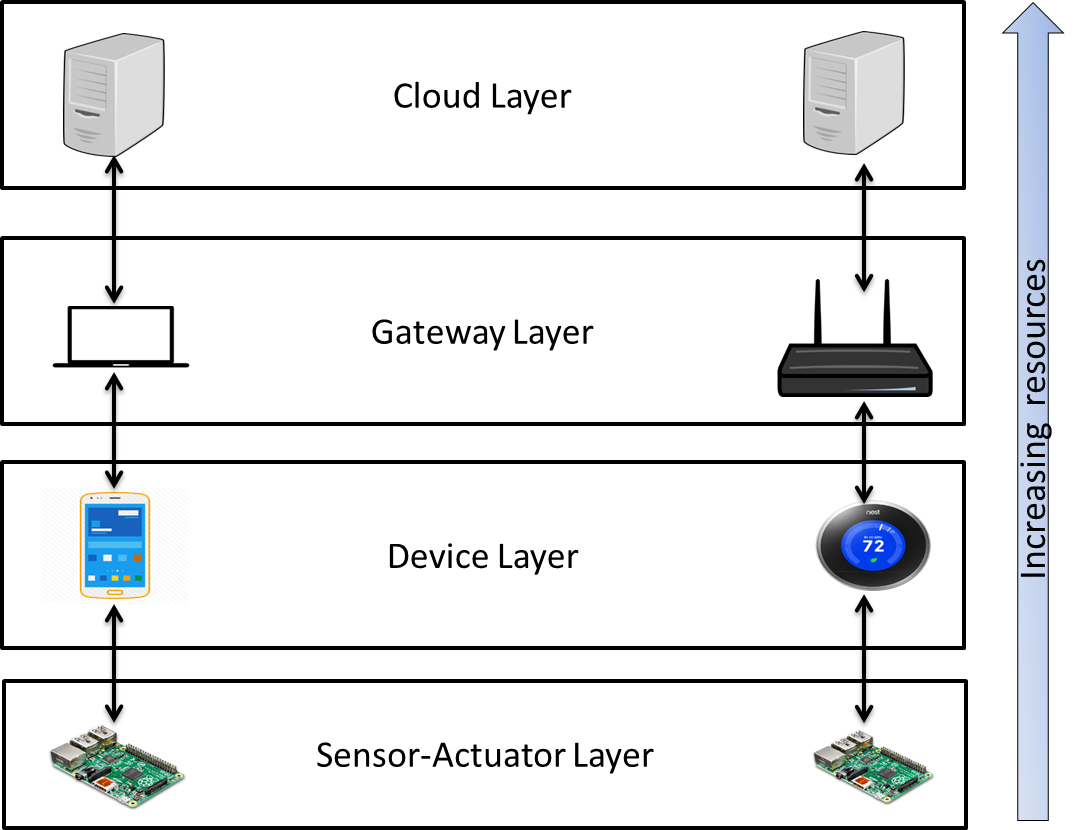
\includegraphics[height=3.0in]{iot_architecture.png}
\end{center}
\caption{IoT Architecture Diagram. The arrows illustrates the interaction between data at various layers on the architecture.}
\label{iot_architecture}

\end{figure}



\section{Comparison of Provenance with Log Data and Metadata}

Provenance data, log data and metadata are key data concepts that often are used interchangeably. We try to address the differences and similarities between provenance data, metadata and log data.

\subsection{Provenance and Metadata}
Metadata and provenance are often considered related but yet subtle distinctions exist. Metadata contains descriptive information about data. Metadata can be considered as provenance when there exists a relationship between objects and they explain the transformation that occurs. In summary,  metadata and provenance are not the same, however an overlap exists. Metadata contains valuable  provenance information but not all metadata is provenance information. 


\subsection{Provenance and Log data}
Log data contains information about the activities of an operating system or processes. Log data can be used as provenance because It contains data trace specific to an application domain. Log files might contain unrelated information such as error messages, warnings which might not be considered as provenance data. Provenance allows for specified collection of information that relates to the change of the internal state of an object. In summary, log data could provide insight to what provenance data to collect. 

\section{Model for representing provenance for IoT}

In order to represent the right kind of provenance information, we need to satisfy the who, where, how, and what of data transformations. Provenance data can be represented using a provenance model in a modeling language such as, PROV\-DM which is represented in serialized form as a JSON object. This model displays the causal relationship of data objects. We propose a model that contains information such as sensor readings, device name, and device information. There are two widely accepted modeling languages for representing provenance, PROV-DM \cite{prov_dm} and  Open Provenance Model \cite{moreau_open_2011} that have been applied in various literature and are considered standard for representing provenance. Details on the provenance models are outlined below.

\subsection{Open Provenance Model (OPM)}

Open Provenance Model \cite{moreau_open_2011} is a specification that was derived as a result of a meeting at the International Provenance and Annotation Workshop (IPAW) in May 2006. OPM was created to address the need of allowing a centralized model for representing provenance data amongst various applications. It allows for interoperability between various provenance applications. The goal of OPM is to represent causality and dependency and also to develop a digital representation of provenance data regardless of if it is produced by a computer system. OPM is represented as a directed acyclic graph which denotes causal dependency between objects. The edges in the graph denotes dependencies with its source denoting effect and its destination denoting cause. The definitions of the edges and their relationships are denoted below: 

\begin{itemize}
\item wasGeneratedBy: This edge denotes a  relationship in which an entity(e,g artifact) is utilized by one or  more entities(e.g process). An entity can use multiple entities so it is important to define the role.  
\item wasControlledBy: This edge outlines a relationship in which an entity caused the creation of another entity.
\item used(Role): This edge denotes that an entity requires the services of another entity in order to execute.
\item wasTriggeredBy: This edge denotes a relationship represents a process that was triggered by another process
\item wasDerrivedFrom: This edge denotes a relationship which indicates that the source needs to have been generated before the destination is generated.
\end{itemize}

 Objects represents the nodes of the relationship graph. There are three object contained in the OPM model: artifact, process, agent. 

\begin{itemize}
\item
artifact: An artifact represents the state of an entity. An artifact is graphically represented by a circle.

\item
Process: A process is an event which takes place at a particular time due to an agent or an artifact. A process is represented by a square object.

\item 
Agent: Agents represents actors that facilitate the execution of a process. An agent is represented by a hexagon in an OPM graph.
\end{itemize}

OPM is used to represent all previous and current actions that have been performed on an entity and  the relationship between each entities contained in the graph. Figure 2 represents an example of an OPM acyclic graph with all of its causal dependencies.  

\begin{figure}[h]
\begin{center}
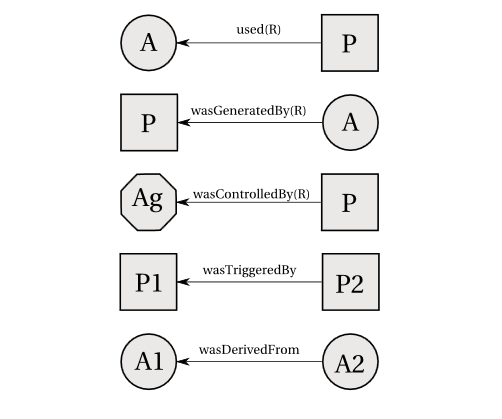
\includegraphics[height=3.0in]{opm_convention.PNG}
\end{center}
\caption{Edges and entities represented in OPM \copyright \cite{moreau_open_2011}}
\label{autom}
\end{figure}

%\begin {center}
%\begin {tikzpicture}[-latex ,auto ,node distance =4 cm and 5cm ,on grid ,
%semithick ,
%state/.style ={ circle ,top color =white , bottom color = processblue!20 ,
%draw,processblue , text=blue , minimum width =1 cm}]
%\node[state] (C)
%{$1$};
%\node[state] (A) [above left=of C] {$0$};
%\node[state] (B) [above right =of C] {$2$};
%\path (A) edge [loop left] node[left] {$1/4$} (A);
%\path (C) edge [bend left =25] node[below =0.15 cm] {$1/2$} (A);
%\path (A) edge [bend right = -15] node[below =0.15 cm] {$1/2$} (C);
%\path (A) edge [bend left =25] node[above] {$1/4$} (B);
%\path (B) edge [bend left =15] node[below =0.15 cm] {$1/2$} (A);
%\path (C) edge [bend left =15] node[below =0.15 cm] {$1/2$} (B);
%\path (B) edge [bend right = -25] node[below =0.15 cm] {$1/2$} (C);
%\end{tikzpicture}
%\end{center}


\subsection{Provenance Data Model (Prov-DM)}

Another model for representing provenance data is the Provenance Data Model (PROV\-DM). PROV-DM is a W3C standardized extension of OPM. Prov-DM is a model that is used to depict causal relationships between entities, activities and agents (digital or physical).  It creates a common model that allows for interchange of provenance information between heterogeneous devices. It contains two major components: types and relations. 


\begin{itemize}

\item Entity: An entity is a physical or digital object. An example of an entity is a file system, a process, or an motor vehicle. An entity may be physical or abstract.

\item Activity: An activity represents some form of action that occurs over a time frame. Actions are acted upon by an agent. An example of an activity is a process opening a file directory, Accessing a remote server.

\item Agent: An agent is a thing that takes ownership of an entity, or performs an activity. An example of an agent is a person, a software product, or a process.
\end{itemize}

The figure below illustrates the various types contained in PROV-DM and their representation. Entities, activities and agents are represented by oval, rectangle and hexagonal shapes respectively.

\begin{figure}[h]
\begin{center}

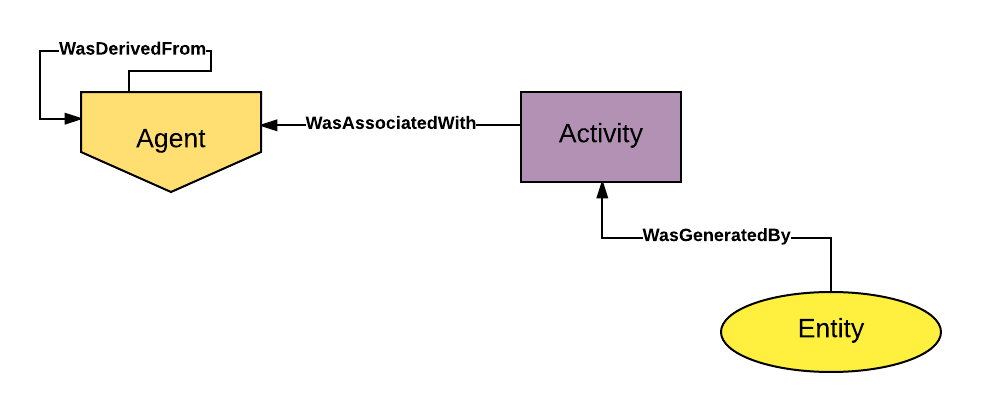
\includegraphics[width=4.0in]{prov_dm_1.PNG}
\end{center}
\caption{Prov-DM respresentation }
\end{figure}

Similar to the OPM, PROV-DM does not keep track of future events. PROV-DM relations are outlined below:


\begin{itemize}
\item wasGeneratedBy: This relation signifies the creation of an entity by an activity. 

\item used: This relation denotes that the functionality of an entity has been adopted by an activity.

\item wasInformedBy: This relation denotes a causality that follows the exchange of two activities.

\item wasDerivedFrom: This relation represents a copy of information from an entity. 

\item wasAttributedTo: This denotes relational dependency to an agent. It is used to denote relationship between entity and agent when the activity that created the agent is unknown.

\item wasAssociatedWith: This relation denotes a direct association to an agent for an activity that occurs.This indicates that an agent plays a role in the creation or modification of the activity.

\item actedOnBehalfOf: This relation denotes assigning authority to perform a particular responsibility to an agent. This could be by itself or to another agent.



\end{itemize}

Some of the difference between OPM and PROV-DM are described below:

\begin{itemize}

\item The main components Artifact, Process and Agent in the OPM model are modified to Entity, Action, and Agent. 

\item Additional causal dependencies such as wasAttributedTo and actedOnBehalfOf were included to represent direct and indirect causal dependencies respectively between agents and entities.

\end{itemize}

%Since PROV-DM is built ontop of OPM and contains easy to understand constructs of types and relations. We are envision are properly represented through the various types and relations, we choose this model to represent provenance data in our IoT architecture instead of OPM. 

\subsection{PROV-JSON}

PROV-JSON is used for representing PROV-DM data in JSON(Javascript Object Notation) format. It contains all of the components and relationships contained in PROV-DM and allows for easy serialization and deserialization. JSON is a lightweight data format which is human readable and easy to parse. Figure \ref{provjson} illustrates a use case for the serialization of PROV-DM to PROV-JSON. PROV-JSON contains key-value pairs and can be considered as an indexed version of PROV-DM. The example depicts the relationship in which s1 tries to access a file (FileB) which was generated by s2. PROV-JSON  contains an entity, activity and agent which is represented as a json object and is identified by their respective ids.  identifiers are optional in PROV-DM but are required for PROV-JSON since json objects contains a key-value pairs, the id's of each object has to be implicitly specified and cannot contain null values. Each object contains fields which assigns additional attributes to the relations (i.e name, type, prov:startTime).  PROV-JSON documents might also contain a prefix object which defines namspaces which are used in the document. In this object is contained a default field which is used to define all of the namespace that contains all other unprefixed namespace.


\begin{figure}[h]
\begin{center}

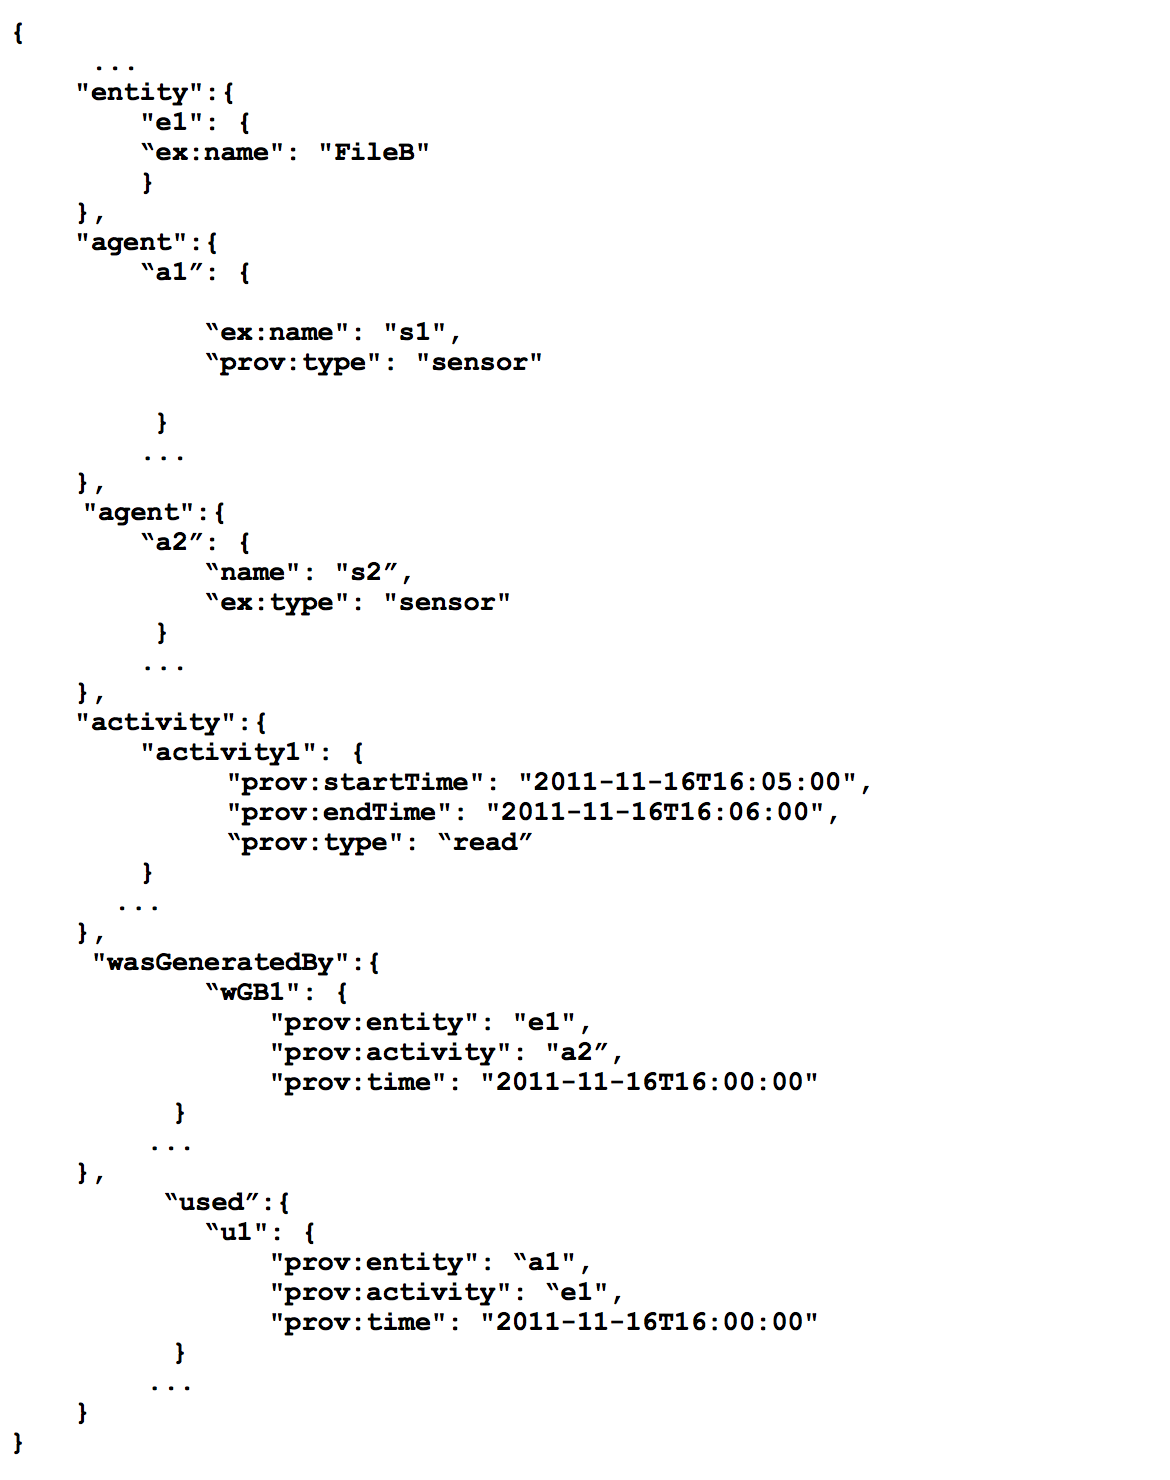
\includegraphics[height=5.7in]{prov_json_edit.png}
\end{center}
\caption{PROV-JSON MODEL \copyright \cite{prov_json}}

\label{provjson}

\end{figure}


\section{Policy Model}

\subsection{eXtensible Access Control Markup Language}
 XACML is an access control policy language that allows the creation and enforcement of policies written in XML. It is a standard specification developed by the Organization of Advancement of Structured Information Standards(OASIS). Since it is written in XML, this framework allows for extensible and flexible policy documents. XACML consists of three major components which are involved in policy generation, evaluation and enforcement. The components of XACML are described below: 
 
 
 \begin{itemize}
 
 \item Policy Administration Point (PAP): This component of XACML
is involved with the generation of policy documents. A Policy document is created by specifications and requirements set aside by an administrator.

 \item Policy Decision Point (PDP): The Policy Decision Point evaluates policies by the request context generated by a user. Based on the request, It generates a response(accept,deny or intermediate) This response is communicated with the Policy Enforcement Point which enforces the response sent by the PDP.


\item Policy Enforcement Point (PEP):  The Policy Enforcement Point generates request context which is sent to the PDP for evaluation. It is also involved with the responsibility of enforcing request based on decision received by the PDP.

 \end{itemize}
 
 
 
 \begin{figure}[h!]
\begin{center}
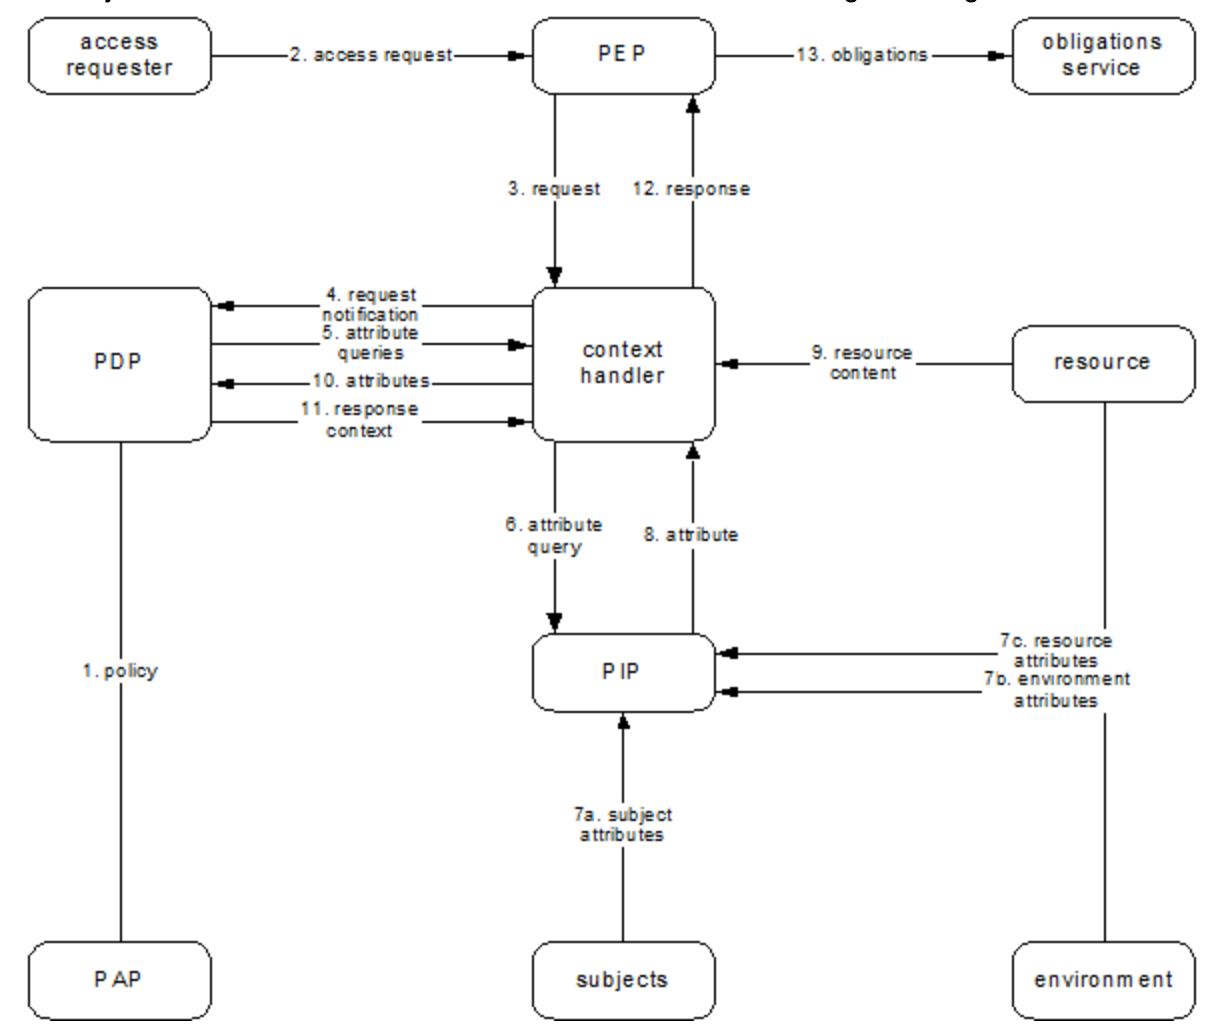
\includegraphics[height=3.5in]{xacml.png}
\caption{Xacml Data-flow diagram  \copyright \cite{xacml}}
\end{center}
\end{figure}
 
%\section{Overview of Relevant Compression techniques}
%
%\subsection{Lossy Compression}
%
%Lossy compression \cite{Sayood:2000:IDC:336428} is a form of data compression in which original data can be reconstructed with some tolerance on loosing some information contained in the original data. This enables higher compression ratio than other compression techniques. Lossy Compression is mostly used in applications that do not contain strict requirements as to loosing some information. An example of a lossless compression application can be seen in an image compression software where the quality of the image is not seen by the naked eye. It is also used in speech transmission. 
%
%\subsection{Lossless Compression}
%Lossless compression \cite{Sayood:2000:IDC:336428} is a data compression technique in which the original data is reconstructed without loss of any information. It can be used by applications which requires that the data is compressed and the original data be identical. An example of such an application that requires lossless compression is text compression.  Any compression that alters the structure of the original text results to a different meaning of the text. For instance, the sentence ``I have a black cat" would have a different meaning if any information is lost from it.
%
%
%
%\subsubsection{Arithmetic Coding}
%
%Arithmetic coding is a form of lossless compression which encodes a stream of characters into a variable size interval between [0,1). A probability is assigned to each characters contained in the string. A cumulative probability is used to calculate the interval of the respective character. Frequent characters are encoded with shorter codes than less frequent characters. 
